% COMP9517 26T2 Group Project Report
% Official CVPR LaTeX template with required page numbers.
\documentclass[10pt,twocolumn,letterpaper]{article}

% Required by the COMP9517 project specification.
\usepackage[pagenumbers]{cvpr}

%% Disable draft TODOs in submitted builds.
\usepackage{booktabs}
\usepackage{graphicx}
\usepackage{microtype}
\usepackage{multirow}
\usepackage{tabularx}
\usepackage{xcolor}
\usepackage{placeins} % \FloatBarrier: keep floats out of later sections


\definecolor{cvprblue}{rgb}{0.21,0.49,0.74}
\usepackage[breaklinks,colorlinks,allcolors=cvprblue]{hyperref}

\def\confName{CVPR}
\def\confYear{2026}

\title{Fine-Grained Species Classification on iNaturalist-2021:\\
Handcrafted Baselines, Scratch and Pretrained CNNs, and Grad-CAM Analysis}

% Authors in role order A--E.
\author{
Xiangze Xue \quad
Zhigeng Qiao \quad
Zhiyang Ding \quad
Yongqi Yang \quad
Xinyan Chen
}

\begin{document}
\maketitle

\begin{abstract}
We study fine-grained 500-species classification on a frozen subset of
iNaturalist-2021. On a balanced 40/10/10 train/validation/test split
(20{,}000 / 5{,}000 / 5{,}000 images; seed~9517), we compare two traditional
pipelines---global colour/LBP/HOG features with a linear SVM objective, and
SIFT Bag-of-Visual-Words with LinearSVC---against deep models trained from
scratch and with ImageNet pretraining (ResNet-18 and EfficientNet-B0). All
methods share the same data manifests and a score-based evaluator reporting
Top-1, Top-5, and macro precision/recall/F1. Pretrained EfficientNet-B0
achieves the best held-out Top-1 accuracy of 76.66\%, far above classical
baselines (4.48\% and 8.86\%) and a scratch ResNet-18 with augmentation
(41.32\%). Grad-CAM analysis of scratch and pretrained networks shows that
correct predictions often attend to organism regions, while fine-grained
confusions persist among visually similar taxa. Controlled ablations isolate
the contributions of descriptors, vocabulary size, data augmentation,
pretraining, and architecture.
\end{abstract}

% =====================================================================
\section{Introduction}
% =====================================================================

Citizen-science imagery makes automated species recognition both useful and
difficult: photographs vary widely in scale, pose, illumination, and
background clutter, while many taxa differ only by subtle local cues
\cite{vanhorn2018inaturalist,vanhorn2021benchmarking}. Platforms such as
iNaturalist accumulate millions of opportunistic observations; reliable
vision systems could assist ecological monitoring, but fine-grained 500-way
classification with only tens of labelled images per species remains
challenging for both classical descriptors and deep networks.

This project evaluates whether classical computer-vision pipelines and modern
convolutional networks can recognise 500 randomly selected iNaturalist
species under a strict train/validation/test protocol. We deliberately
contrast global handcrafted features, local Bag-of-Visual-Words histograms,
scratch-trained CNNs, and ImageNet-pretrained CNNs on the \emph{same} frozen
splits, then interpret deep predictions with Grad-CAM.

We make three contributions:
\begin{enumerate}
  \item A frozen, audited 500-class Dataset~v1.0 with shared score-based
  evaluation so handcrafted and deep methods are compared fairly.
  \item A method suite covering global and local handcrafted pipelines; a
  ResNet-18 trained from scratch with a controlled augmentation ablation; and
  ImageNet-pretrained ResNet-18 and EfficientNet-B0.
  \item Confusion analysis and Grad-CAM visualisations comparing attention
  across scratch and pretrained models on matched images.
\end{enumerate}

The remainder of this report reviews related work, details methods and
hyperparameters, presents quantitative and qualitative results, discusses
limitations, and concludes.

% =====================================================================
\section{Literature Review}
% =====================================================================

\paragraph{Fine-grained natural-world recognition.}
The iNaturalist benchmarks emphasise long-tailed, fine-grained categories
photographed in the wild \cite{vanhorn2018inaturalist,vanhorn2021benchmarking}.
Performance gaps between simple baselines and representation-learning models
motivate reporting both classical and deep approaches under identical splits.

\paragraph{Handcrafted descriptors.}
Colour histograms, Local Binary Patterns (LBP) \cite{ojala2002multiresolution},
and Histograms of Oriented Gradients (HOG) \cite{dalal2005histograms} provide
interpretable global colour, texture, and shape cues. Scale-Invariant Feature
Transform (SIFT) keypoints \cite{lowe2004distinctive} aggregated into a
Bag-of-Visual-Words (BoVW) histogram \cite{csurka2004visual} capture
repeatable local patterns but discard spatial layout. Linear support-vector
machines remain a strong classical classifier for high-dimensional sparse or
dense features \cite{cortes1995support,pedregosa2011scikit}; Random Forests
offer a non-linear alternative \cite{breiman2001random}.

\paragraph{Deep residual and efficient CNNs.}
Residual networks use identity shortcuts to learn residual functions, easing
optimisation of deeper models \cite{he2016deep}. We use ResNet-18 as a
moderate-capacity scratch baseline that remains practical to retrain on one
GPU. Data augmentation (e.g., cropping and horizontal flipping) exposes the
network to varied views of each training image and can reduce overfitting when
labels are preserved \cite{shorten2019augmentation}; we measure this effect
with a controlled ablation rather than assuming it helps. Training uses a
cosine learning-rate schedule \cite{loshchilov2017sgdr}. EfficientNet compounds
depth, width, and resolution and is a strong ImageNet transfer baseline
\cite{tan2019efficientnet}. ImageNet pretraining remains a dominant inductive
bias when labelled data per class are limited \cite{krizhevsky2012imagenet}.

\paragraph{Explainability.}
Grad-CAM produces class-discriminative heatmaps by weighting convolutional
feature maps with gradients of a target class score
\cite{selvaraju2017gradcam}. We apply it to scratch and pretrained models on
matched test images to ask whether correct predictions attend to the organism,
how high-confidence errors behave, and whether pretraining changes attention
on confusable Accipitridae pairs. We treat Grad-CAM as an interpretability aid
rather than causal proof that altering a highlighted region would flip the
label.

% =====================================================================
\section{Methods}
% =====================================================================

\subsection{Dataset and experimental protocol}
\label{sec:data}

We construct a 500-species subset of iNaturalist-2021 with random seed
\textbf{9517}. For each species, 40 images from the official \texttt{train\_mini}
split form the training set and 10 form validation; 10 images from the
official iNat validation split form the held-out \textbf{test} set (following
the project specification). Totals are 20{,}000 / 5{,}000 / 5{,}000 images with
balanced class frequencies. Contiguous \texttt{class\_index} values $0\ldots499$
are stored with taxonomy fields (kingdom through species). Structural and
SHA-256 audits removed one byte-identical cross-split duplicate via a
deterministic category replacement that preserves indices. All methods consume
the frozen Dataset~v1.0 CSV manifests with relative image paths.

Hyperparameters are selected on validation only. After freezing
preprocessing, architecture, and classifier settings, the test set is
evaluated \textbf{once}. Reported metrics are Top-1 and Top-5 accuracy, macro
precision/recall/F1, and wall-clock training and inference times. For this
single-label task, overall accuracy equals Top-1. A shared evaluator consumes
an $N\times500$ score matrix and emits identical metric definitions, per-image
Top-5 predictions, and a $500\times500$ confusion matrix for every method,
so classical and deep pipelines are scored the same way.

\subsection{Global handcrafted features (Method A)}
\label{sec:method-a}

Each image is resized to $128\times128$. We concatenate (i)~a 57-D colour
descriptor (16-bin HSV histograms plus RGB mean/std/skewness), (ii)~uniform
LBP ($P{=}8$, $R{=}1$) pooled on a $4\times4$ grid (160-D), and (iii)~HOG with
9 orientations, $16\times16$ cells, and $2\times2$ blocks (1{,}764-D), yielding
a 1{,}981-D vector. Features are standardised on the training set.
Classification uses a multiclass linear hinge-loss (SVM) objective optimised
with averaged SGD ($C{=}1$, $\alpha = 1/(C\,N_{\mathrm{train}})$, seed~9517),
chosen because direct one-vs-rest linear SVM fitting was impractically slow for
20{,}000 images and 500 classes. We ablate input resolution, individual
descriptors, and $C$ on validation, changing one factor at a time; the 20-class
pilot is used only to verify implementation and is excluded from final claims.

\subsection{SIFT Bag-of-Visual-Words (Method B)}
\label{sec:method-b}

Images are converted to grayscale and resized so that the longer side is at
most 512 pixels. OpenCV SIFT extracts descriptors
($\texttt{contrastThreshold}{=}0.04$). A visual vocabulary is fit with
MiniBatchKMeans on up to 500k training descriptors only (seed~9517). Each
image is encoded as a hard-assignment BoVW histogram, TF--IDF weighted (fit on
train), and $\ell_2$-normalised. We train one-vs-rest LinearSVC ($C{=}1$,
\texttt{dual=false}) and compare a capacity-limited Random Forest (100 trees,
\texttt{max\_depth}{=}30). Vocabulary sizes $K\in\{500,1000,2000\}$ are
compared; $K$ is selected by validation macro-F1.

\subsection{Scratch ResNet-18 (Method C)}
\label{sec:method-c}

We use torchvision ResNet-18 with \texttt{weights=None} (no pretrained
parameters) and replace the classifier with a 500-way linear head
\cite{he2016deep}. Images are converted to RGB and normalised with ImageNet
channel mean/std; this only sets input scale and does \emph{not} transfer
learned weights. Training uses cross-entropy and SGD (lr 0.05, momentum 0.9,
weight decay $10^{-4}$), cosine annealing for up to 100 epochs
\cite{loshchilov2017sgdr}, batch size 128, AMP, and seed~9517 reset before
each model construction so C0 and C1 share the same initial weights. Early
stopping uses patience 15 (min.\ improvement $10^{-4}$) on validation
macro-F1; the best checkpoint is selected by that metric, and the test set is
used only after freezing.

The two runs differ \textbf{only} in the training transform (no colour
jitter): \textbf{C0} uses \texttt{Resize(256)+CenterCrop(224)}; \textbf{C1}
uses \texttt{RandomResizedCrop(224)+RandomHorizontalFlip}. Validation and
test always use deterministic resize and centre crop. Dataset manifests,
architecture, optimiser, scheduler, batch size, epoch budget, checkpoint
rule, and evaluation code are otherwise identical, so the performance gap is
attributed to random crop and flip under seed~9517.

\subsection{Pretrained CNNs (Method D)}
\label{sec:method-d}

We fine-tune ImageNet-pretrained ResNet-18 and EfficientNet-B0
\cite{tan2019efficientnet} on the same data, replacing the final layer with a
500-class head. Training uses SGD with the same nominal learning-rate
settings as Method~C (lr 0.05, momentum 0.9, weight decay $10^{-4}$, cosine
schedule, batch size 128) and standard random-crop/flip augmentation, so the
main contrasts versus C1 are initialisation (scratch vs.\ pretrained) and, for
EfficientNet-B0, architecture under matched data. Best epochs by validation
performance are 85 (ResNet-18) and 84 (EfficientNet-B0). This isolates the
value of transfer learning after establishing a strong scratch reference, then
asks whether a more recent efficient CNN further improves transfer accuracy.

\subsection{Grad-CAM error analysis (Method E)}
\label{sec:method-e}

Grad-CAM \cite{selvaraju2017gradcam} is applied to C1 (scratch ResNet-18),
pretrained ResNet-18, and EfficientNet-B0 on matched test images under
identical preprocessing (\texttt{Resize(256)}, \texttt{CenterCrop(224)},
ImageNet normalisation) with models in evaluation mode. Target layers are
\texttt{layer4[-1]} for both ResNet-18 variants and \texttt{features[-1]} for
EfficientNet-B0; heatmaps explain the \emph{predicted} class so that we
visualise the decision the model actually made. The same image IDs are reused
across models to keep the qualitative comparison controlled. Cases are
selected by rule, not only visual appeal: high-confidence correct predictions,
high-confidence errors, and examples from the frequent Imperial Eagle
(\emph{Aquila heliaca}) vs.\ European Honey-buzzard (\emph{Pernis apivorus})
confusion pair. Because ResNet and EfficientNet target layers are not
architecturally matched, cross-architecture comparisons remain qualitative.

\subsection{Hyperparameter summary}

Table~\ref{tab:hparams} lists the main frozen settings used for the final
reported models. All deep runs share seed~9517 and select checkpoints by
validation performance (macro-F1 for Methods~C/A-style selection rules;
pretrained runs use the saved best epoch recorded in each config).

\begin{table*}[t]
\centering
\footnotesize
\setlength{\tabcolsep}{3.5pt}
\begin{tabular}{@{}llp{0.58\linewidth}@{}}
\toprule
ID & Family & Key hyperparameters \\
\midrule
A & Global + SVM-obj.\ SGD
  & Resize $128$; Colour(57)+LBP(160)+HOG(1764); $C{=}1$; avg.\ SGD; seed~9517 \\
B & SIFT-BoVW + LinearSVC
  & max side 512; MiniBatchKMeans $K{=}2000$; TF--IDF+$\ell_2$; LinearSVC $C{=}1$, \texttt{dual=false} \\
C1 & Scratch ResNet-18
  & RandomResizedCrop/Flip; SGD lr 0.05, mom.\ 0.9, wd $10^{-4}$; cosine; BS 128; $\le$100 ep.; patience 15 \\
D-R18 & Pretrained ResNet-18
  & ImageNet weights; SGD as above; best epoch 85; train $\approx$2689~s \\
D-B0 & Pretrained EfficientNet-B0
  & ImageNet weights; SGD as above; best epoch 84; train $\approx$4664~s \\
\bottomrule
\end{tabular}
\caption{Frozen hyperparameters for final reported models.}
\label{tab:hparams}
\end{table*}

% =====================================================================
\section{Experimental Results}
% =====================================================================

\subsection{Main comparison on the held-out test set}

Table~\ref{tab:main} summarises frozen final-model test metrics on all 5{,}000
images. EfficientNet-B0 pretrained is strongest (76.66\% Top-1), followed by
pretrained ResNet-18 (65.10\%), scratch ResNet-18 with augmentation (41.32\%),
SIFT-BoVW (8.86\%), and global colour/LBP/HOG (4.48\%). Chance Top-1 is
$0.2\%$. Table~\ref{tab:gaps} summarises validation--test Top-1 gaps.

\begin{table}[t]
\centering
\footnotesize
\setlength{\tabcolsep}{3.5pt}
\begin{tabular}{@{}lcccc@{}}
\toprule
Method & Top-1 & Top-5 & Macro-F1 & Macro-P \\
\midrule
A Colour+LBP+HOG + lin.\ SVM & 4.48 & 12.16 & 3.99 & 4.90 \\
B SIFT-BoVW SVM ($K{=}2000$) & 8.86 & 17.80 & 7.71 & 7.41 \\
C1 Scratch R18 + aug & 41.32 & 64.18$^\ast$ & 40.45 & 41.40 \\
D ResNet-18 pretrained & 65.10 & 83.34 & 64.42 & 66.01 \\
D EfficientNet-B0 pretrained & \textbf{76.66} & \textbf{90.50} & \textbf{76.20} & \textbf{77.63} \\
\bottomrule
\end{tabular}
\caption{Held-out test metrics (\%). Macro-P is macro precision. Overall
accuracy equals Top-1. Numbers are from the shared group evaluator on
Dataset~v1.0. $^\ast$C1 frozen metrics JSON reports Top-5 $64.16\%$; the
shared NPZ evaluator yields $64.18\%$.}
\label{tab:main}
\end{table}

\begin{table}[t]
\centering
\footnotesize
\setlength{\tabcolsep}{3pt}
\begin{tabular}{@{}lccc@{}}
\toprule
Method & Val Top-1 & Test Top-1 & Gap (pp) \\
\midrule
A Combined + SVM & 4.80 & 4.48 & $-0.32$ \\
B SIFT-BoVW SVM & 9.08 & 8.86 & $-0.22$ \\
C1 Scratch R18 + aug & 40.90 & 41.32 & $+0.42$ \\
D ResNet-18 pretrained & 62.80 & 65.10 & $+2.30$ \\
D EfficientNet-B0 & 75.96 & 76.66 & $+0.70$ \\
\bottomrule
\end{tabular}
\caption{Validation vs.\ test Top-1 (\%). Gap $=$ test $-$ validation.}
\label{tab:gaps}
\end{table}

\subsection{Traditional-method ablations}

\paragraph{Global descriptors.}
At $128\times128$ and $C{=}1$, Combined colour+LBP+HOG beats each descriptor
alone on validation (Table~\ref{tab:a-desc}): Top-1 rises from 2.84\% (HOG)
to 4.80\% (Combined). Under HOG-only settings, $128\times128$ outperforms
$224\times224$ in Top-1 and macro-F1 while fitting in roughly one third the
time (Table~\ref{tab:a-res}). With Combined features, $C{=}1$ is strongest
among $\{0.01,0.1,1,10\}$ (Table~\ref{tab:a-c}). Paired McNemar tests on
validation support these choices. The frozen model reaches 4.48\% Top-1 /
12.16\% Top-5 on test, close to validation (4.80\% / 12.54\%).
Figure~\ref{fig:a-ablation} summarises the sweeps;
Figure~\ref{fig:a-conf} shows frequent confusion pairs;
Figure~\ref{fig:a-cases} shows representative successes and failures.

\begin{table}[t]
\centering
\footnotesize
\setlength{\tabcolsep}{3pt}
\begin{tabular}{@{}lcccc@{}}
\toprule
Descriptor & Dim & Val Top-1 & Val Top-5 & Val F1 \\
\midrule
Colour & 57 & 2.16 & 7.70 & 1.62 \\
LBP & 160 & 2.50 & 7.58 & 1.78 \\
HOG & 1{,}764 & 2.84 & 8.06 & 2.48 \\
Combined & 1{,}981 & \textbf{4.80} & \textbf{12.54} & \textbf{4.25} \\
\bottomrule
\end{tabular}
\caption{Method~A descriptor ablation on validation ($128\times128$, $C{=}1$).}
\label{tab:a-desc}
\end{table}

\begin{table}[t]
\centering
\footnotesize
\begin{tabular}{@{}lcccc@{}}
\toprule
Resolution & Dim (HOG) & Top-1 & Macro-F1 & Fit time \\
\midrule
\textbf{128} & 1{,}764 & \textbf{2.84} & \textbf{2.48} & \textbf{265~s} \\
224 & 6{,}084 & 2.32 & 2.08 & 807~s \\
\bottomrule
\end{tabular}
\caption{Method~A resolution ablation (HOG only, $C{=}1$; validation \%).}
\label{tab:a-res}
\end{table}

\begin{table}[t]
\centering
\footnotesize
\begin{tabular}{@{}lccc@{}}
\toprule
$C$ & Top-1 & Top-5 & Macro-F1 \\
\midrule
0.01 & 3.48 & 9.52 & 1.78 \\
0.1 & 4.06 & 11.00 & 2.74 \\
\textbf{1} & \textbf{4.80} & \textbf{12.54} & \textbf{4.25} \\
10 & 3.90 & 11.78 & 3.89 \\
\bottomrule
\end{tabular}
\caption{Method~A regularisation ablation (Combined, $128\times128$;
validation \%).}
\label{tab:a-c}
\end{table}

\begin{figure}[t]
\centering
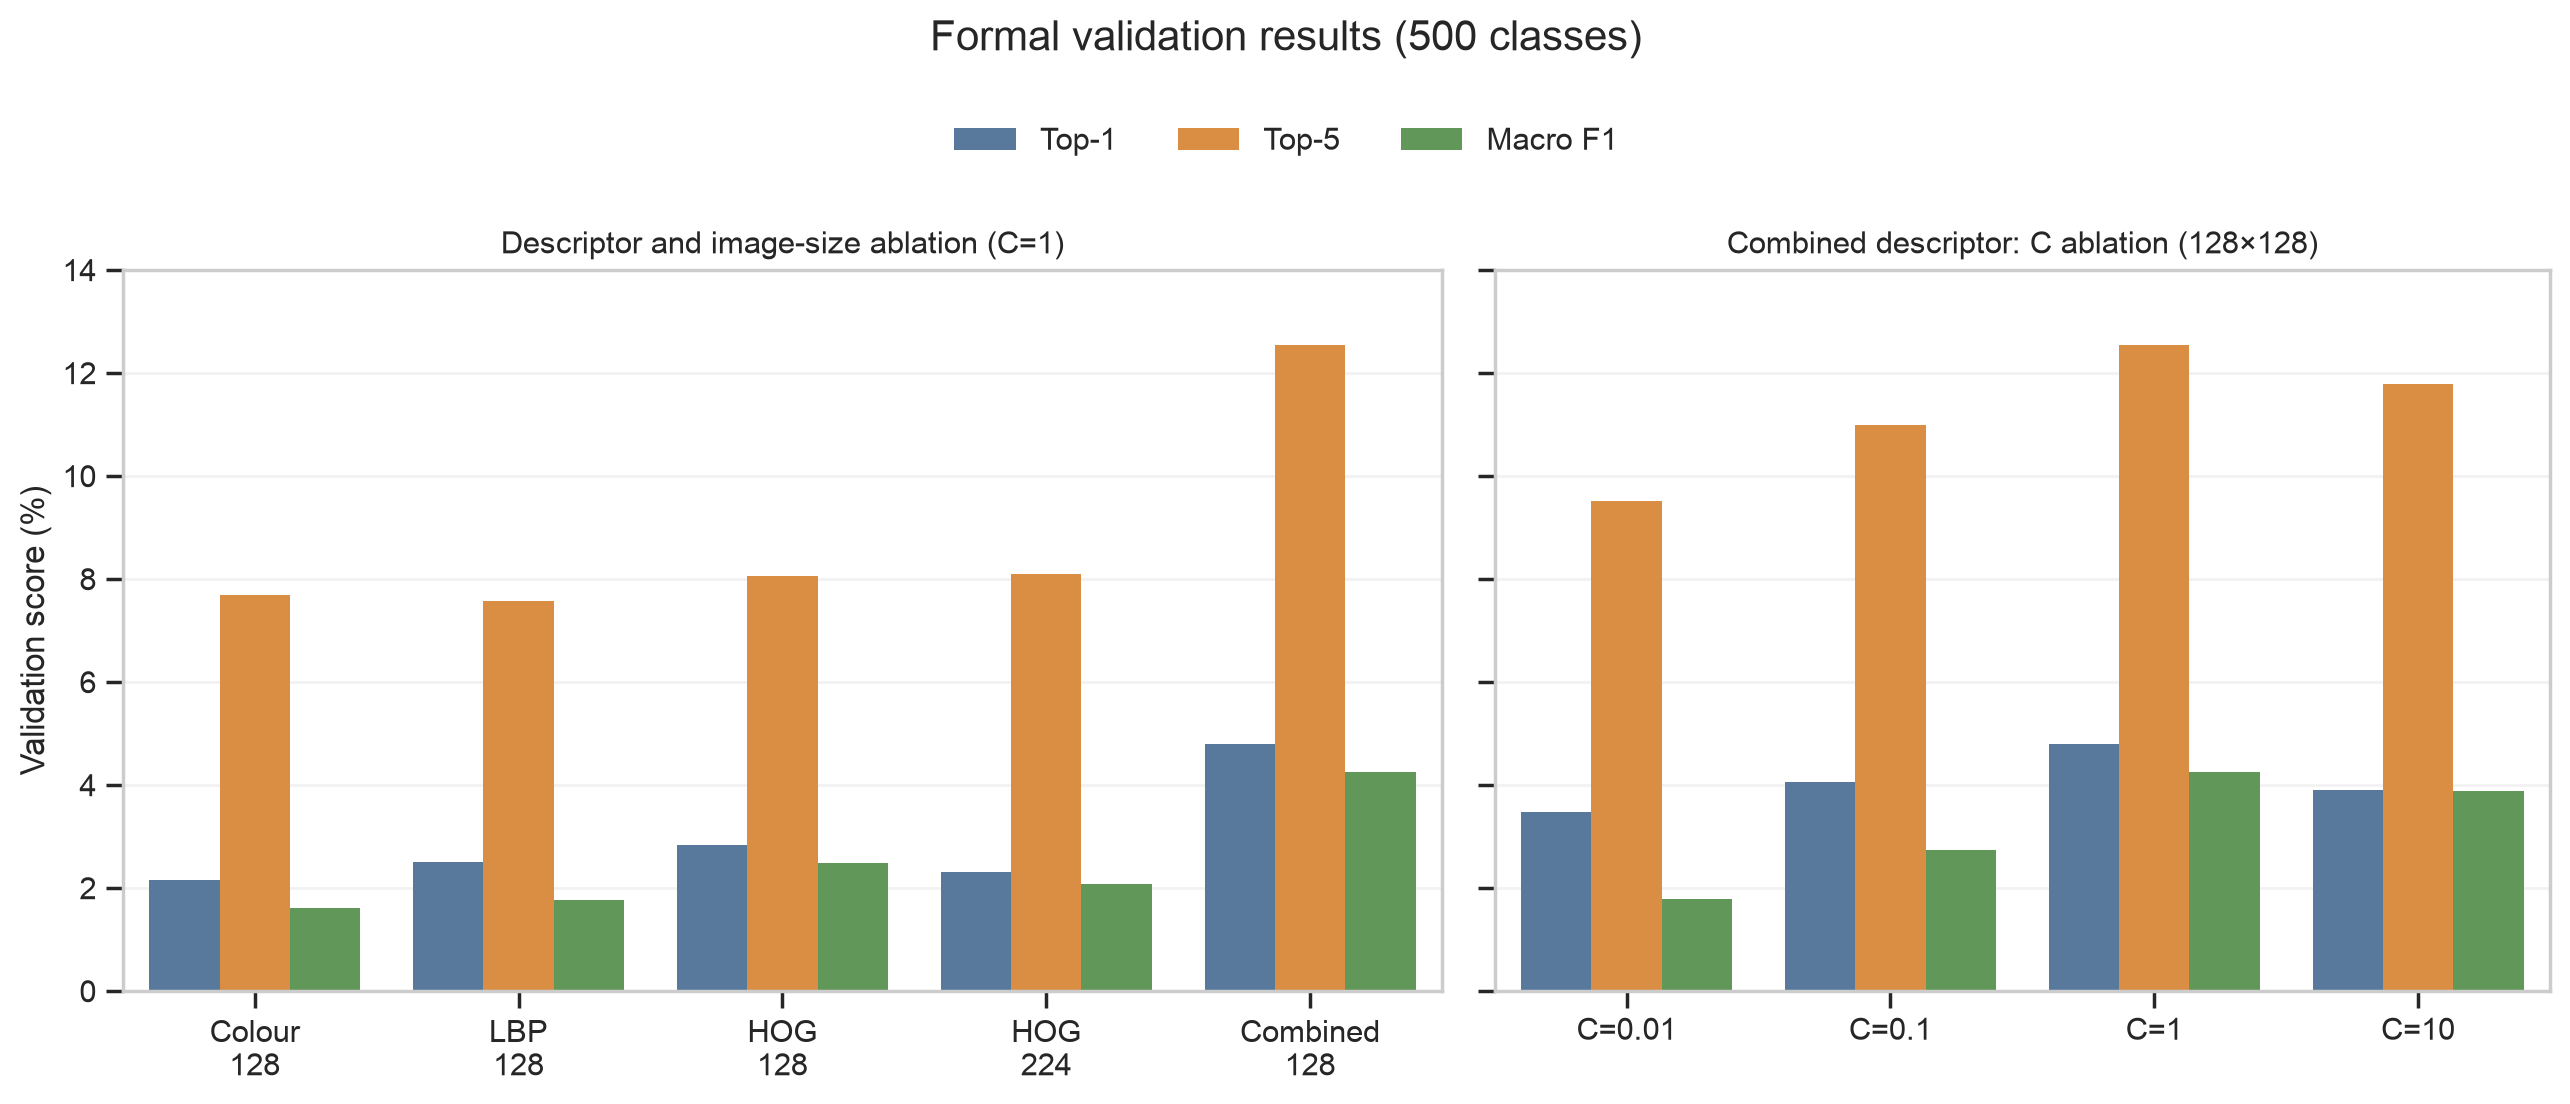
\includegraphics[width=\linewidth]{figures/a_validation_ablation.png}
\caption{Method~A validation ablations (descriptor, resolution, and $C$).}
\label{fig:a-ablation}
\end{figure}

\begin{figure}[t]
\centering
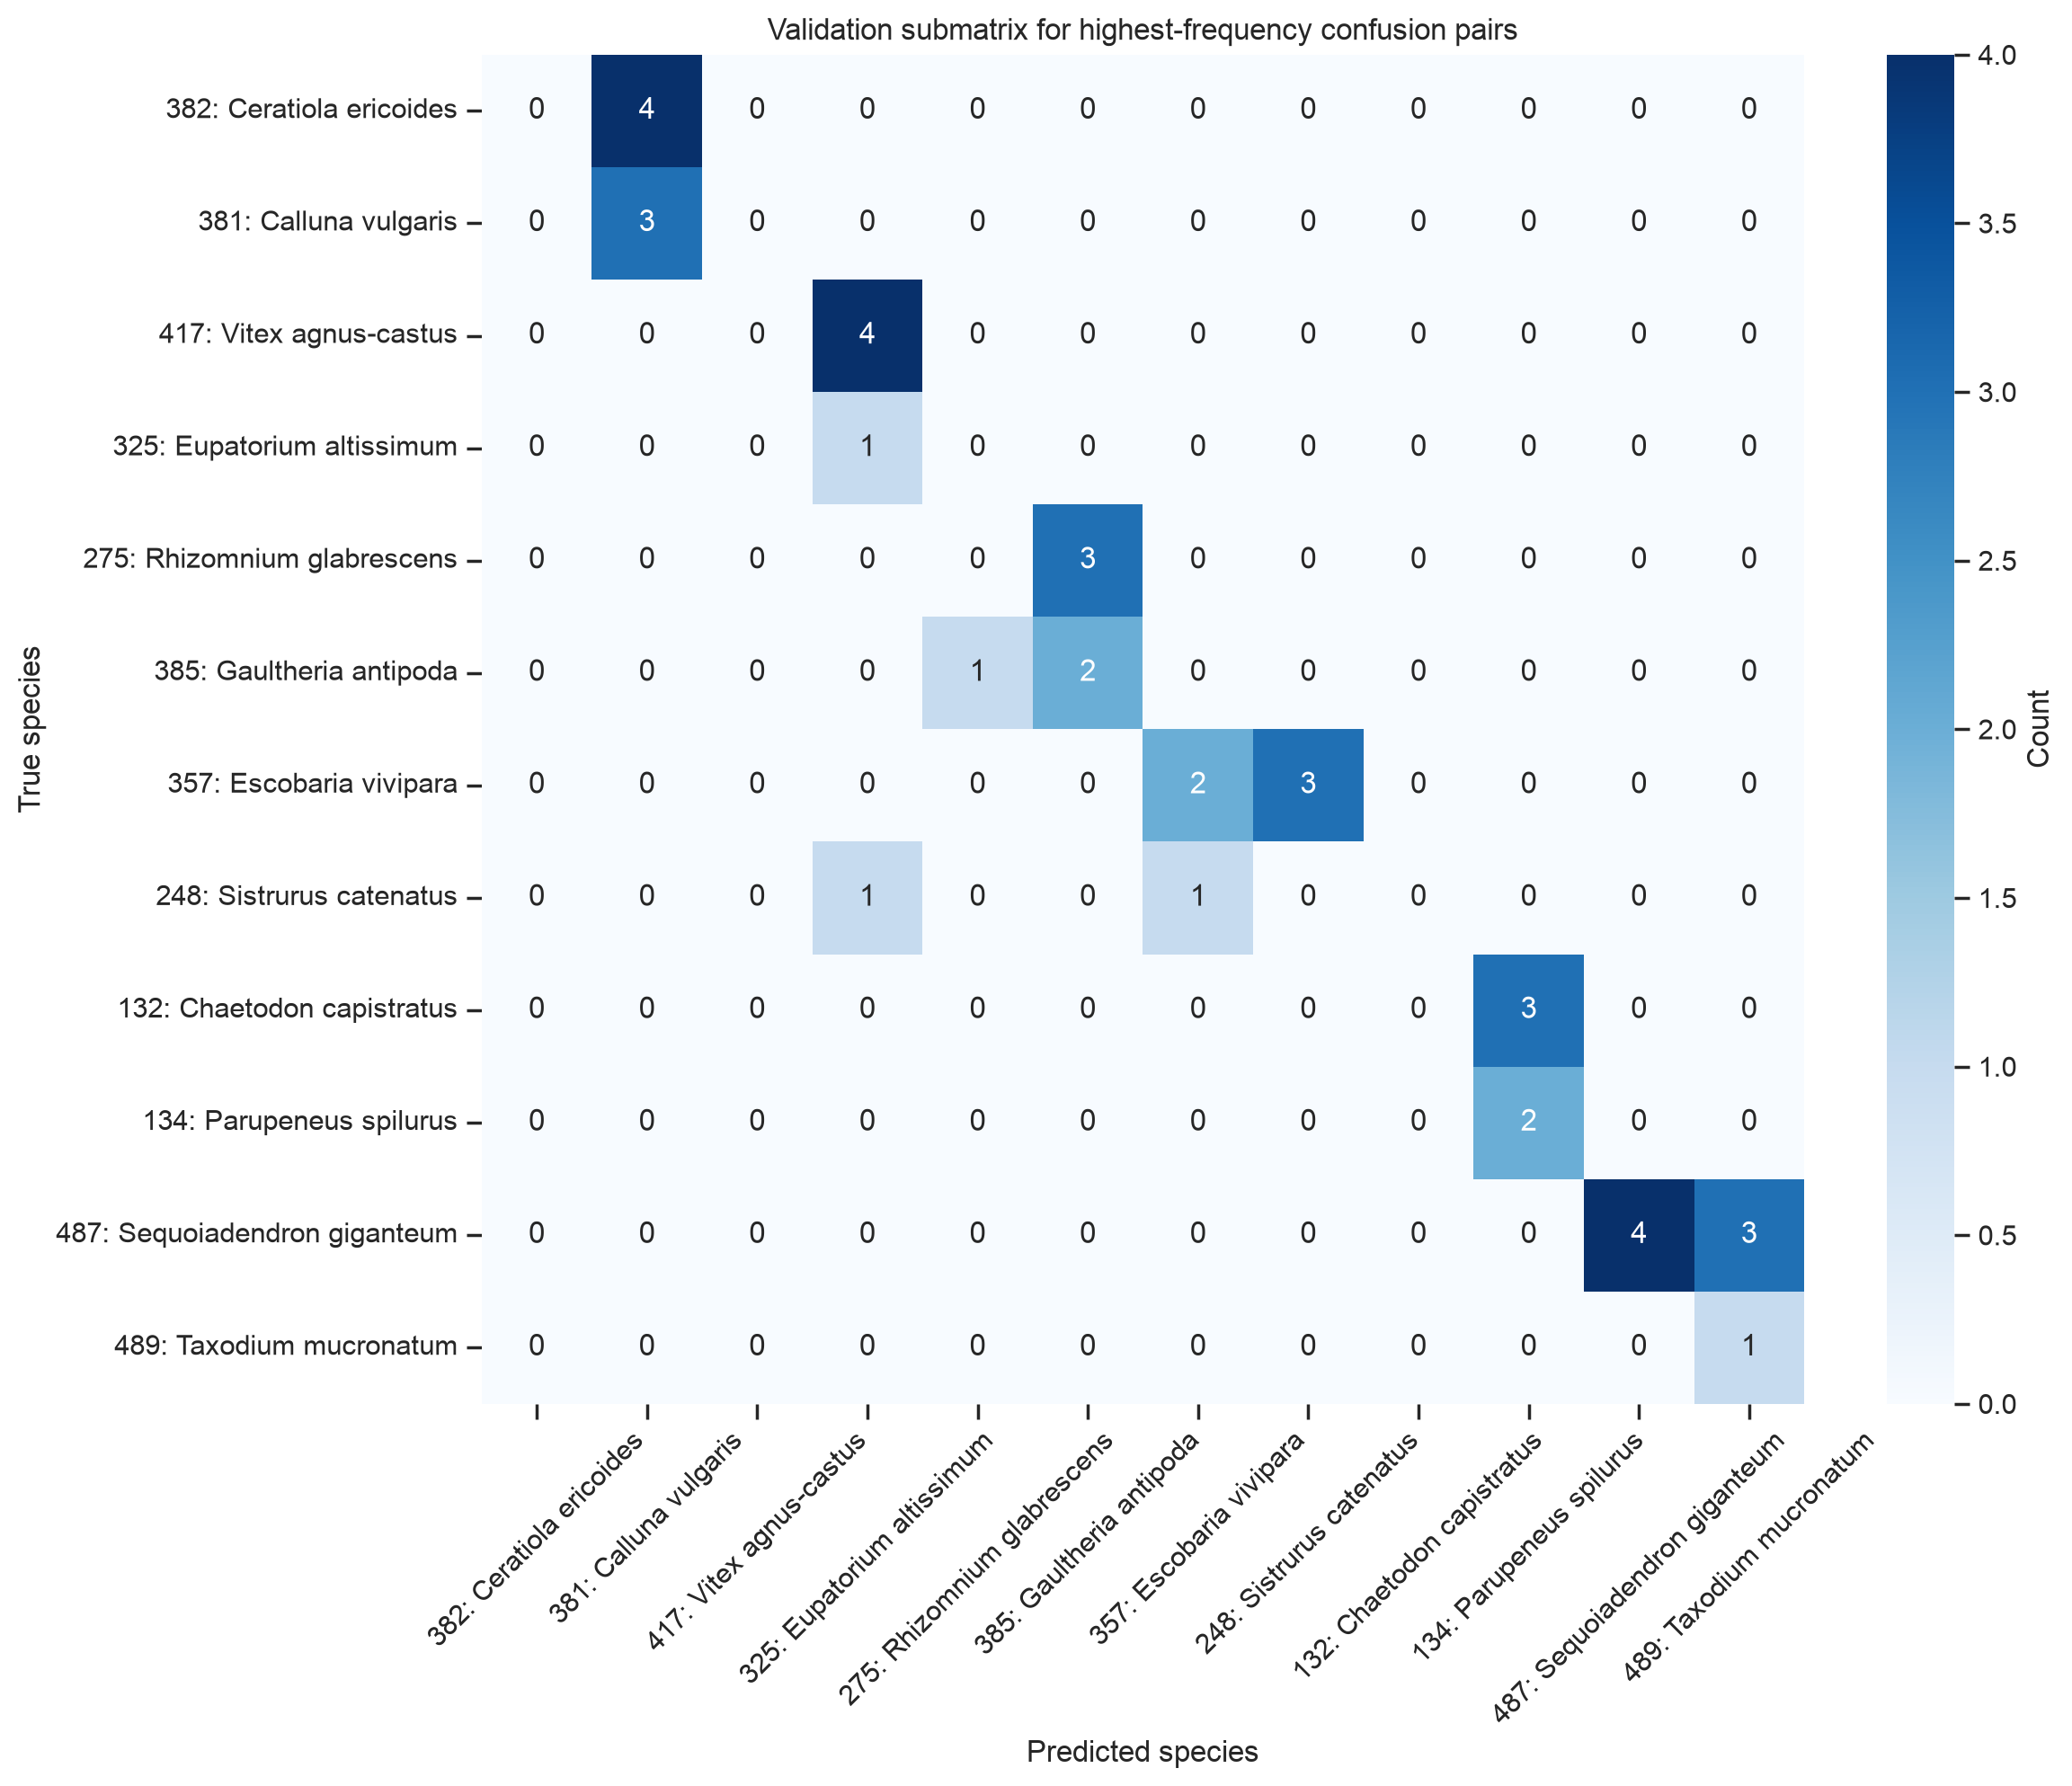
\includegraphics[width=0.95\linewidth]{figures/a_confusion_submatrix.png}
\caption{Method~A readable validation confusion submatrix among frequent pairs.}
\label{fig:a-conf}
\end{figure}

\begin{figure}[t]
\centering
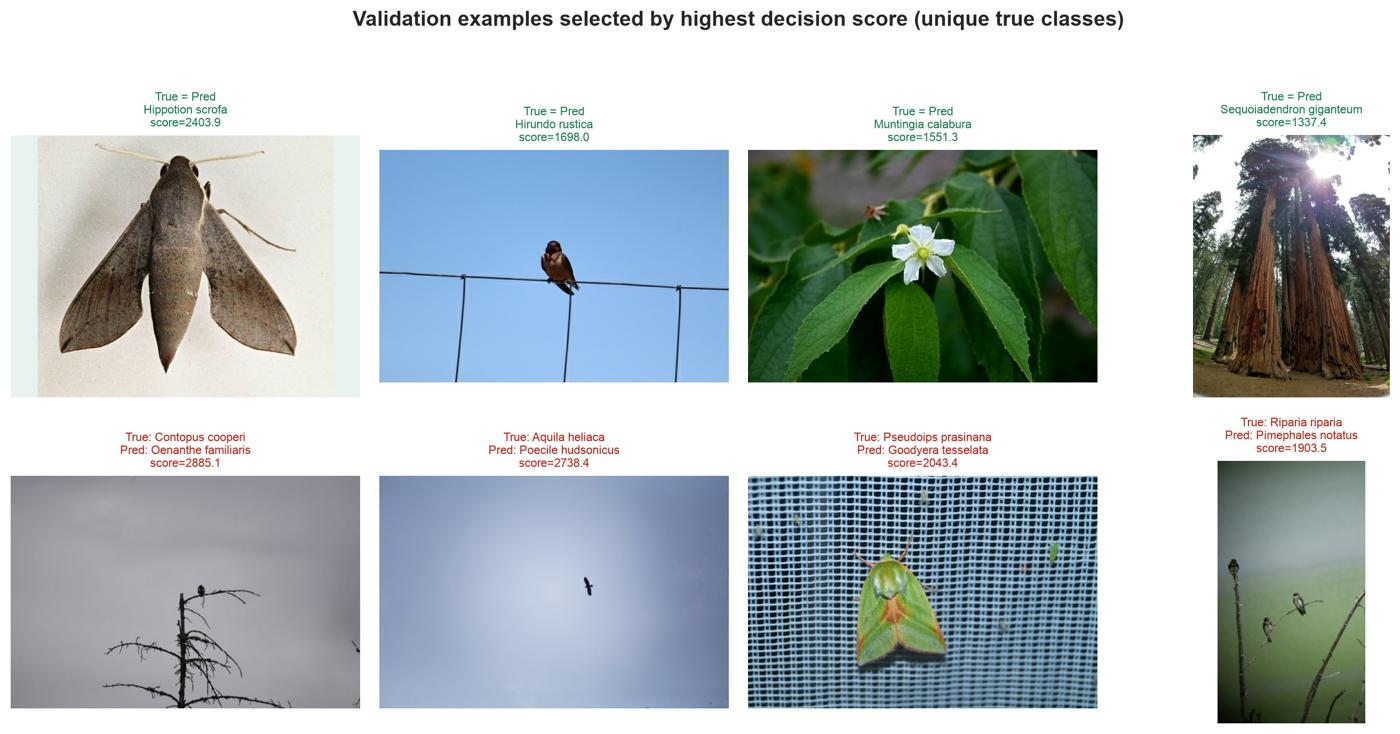
\includegraphics[width=\linewidth]{figures/a_success_failure_cases.jpg}
\caption{Method~A qualitative validation cases: high-scoring correct predictions
(top) versus high-scoring errors (bottom). Failures often show small subjects
or dominant background texture.}
\label{fig:a-cases}
\end{figure}

\paragraph{BoVW vocabulary size.}
Table~\ref{tab:bovw} shows LinearSVC results for $K\in\{500,1000,2000\}$.
Validation selects $K{=}2000$ (macro-F1 7.90\%). Gains over $K{=}500$ are
modest, suggesting that orderless local histograms---not vocabulary
granularity alone---limit accuracy. On the same $K{=}1000$ features, a
depth-limited Random Forest trails LinearSVC substantially (test Top-1
2.98\% vs.\ 8.80\%), so we report LinearSVC as the primary traditional local
baseline. Relative to Method~A, BoVW roughly doubles test Top-1, confirming
that local keypoints add signal beyond global colour/texture/shape, while
remaining far below CNNs. Table~\ref{tab:b-clf} compares classifiers on the
same $K{=}1000$ histograms.

\begin{table}[t]
\centering
\footnotesize
\begin{tabular}{@{}lccccc@{}}
\toprule
$K$ & Val Top-1 & Val F1 & Test Top-1 & Test Top-5 & Test F1 \\
\midrule
500 & 8.28 & 6.54 & 8.82 & 18.68 & 7.07 \\
1000 & 8.66 & 7.47 & 8.80 & 18.82 & 7.46 \\
\textbf{2000} & \textbf{9.08} & \textbf{7.90} & \textbf{8.86} & 17.80 & \textbf{7.71} \\
\bottomrule
\end{tabular}
\caption{Method~B vocabulary ablation (LinearSVC; metrics in \%).}
\label{tab:bovw}
\end{table}

\begin{table}[t]
\centering
\footnotesize
\begin{tabular}{@{}lccc@{}}
\toprule
Classifier (same $K{=}1000$ feats) & Test Top-1 & Top-5 & Macro-F1 \\
\midrule
LinearSVC & \textbf{8.80} & \textbf{18.82} & \textbf{7.46} \\
RF (100 trees, max depth 30) & 2.98 & 7.90 & 2.27 \\
\bottomrule
\end{tabular}
\caption{Method~B classifier comparison on shared $K{=}1000$ BoVW features
(test \%). The RF is capacity-limited for disk/runtime reasons.}
\label{tab:b-clf}
\end{table}

\subsection{Scratch training and augmentation}

Table~\ref{tab:aug} and Figure~\ref{fig:c-curves} compare C0 and C1 on an
RTX~4080 (PyTorch 2.12.1). Training time sums training epochs only; test
inference is a full 5{,}000-image evaluation pass. C1 improves test Top-1 by
19.70 percentage points, Top-5 by 19.92 points, and macro-F1 by 19.03 points.
Validation and test stay close (C0: 21.90\% / 21.62\% Top-1; C1: 40.90\% /
41.32\%), so model selection does not appear to overfit the validation split.

\paragraph{Training dynamics.}
C0 reaches 99.99\% training Top-1 near zero training loss by its best epoch,
yet peaks at only 22.11\% validation macro-F1 and stops at epoch 36 after
patience is exhausted. C1 fits more slowly: best checkpoint at epoch 87 with
91.47\% training Top-1 and 40.17\% validation macro-F1. Lower training
accuracy with much higher validation performance is consistent with
augmentation as a strong regulariser \cite{shorten2019augmentation}.

\paragraph{Top-5 note.}
The shared group evaluator reports C1 test Top-5 as 64.18\%, while the frozen
C1 metrics JSON reports 64.16\%. One test image has an exact logit tie at the
fifth-ranked boundary; NumPy stable sorting and \texttt{torch.topk} disagree
on that slot. Top-1 and all macro metrics match. Table~\ref{tab:main} uses
the shared-evaluator 64.18\%; Table~\ref{tab:aug} keeps the frozen 64.16\%.

\begin{table}[t]
\centering
\footnotesize
\setlength{\tabcolsep}{2.5pt}
\resizebox{\columnwidth}{!}{%
\begin{tabular}{@{}lcccccc@{}}
\toprule
Run & Top-1 & Top-5 & Macro-F1 & Best ep. & Train & Test infer. \\
\midrule
C0 no random aug & 21.62 & 44.24 & 21.42 & 21 & 13.4~min & 5.18~s \\
C1 + crop/flip & \textbf{41.32} & \textbf{64.16} & \textbf{40.45} & 87 & 34.9~min & 6.77~s \\
\bottomrule
\end{tabular}%
}
\caption{Method~C augmentation ablation (frozen C0/C1 metrics JSON; \%).}
\label{tab:aug}
\end{table}

\begin{figure}[t]
\centering
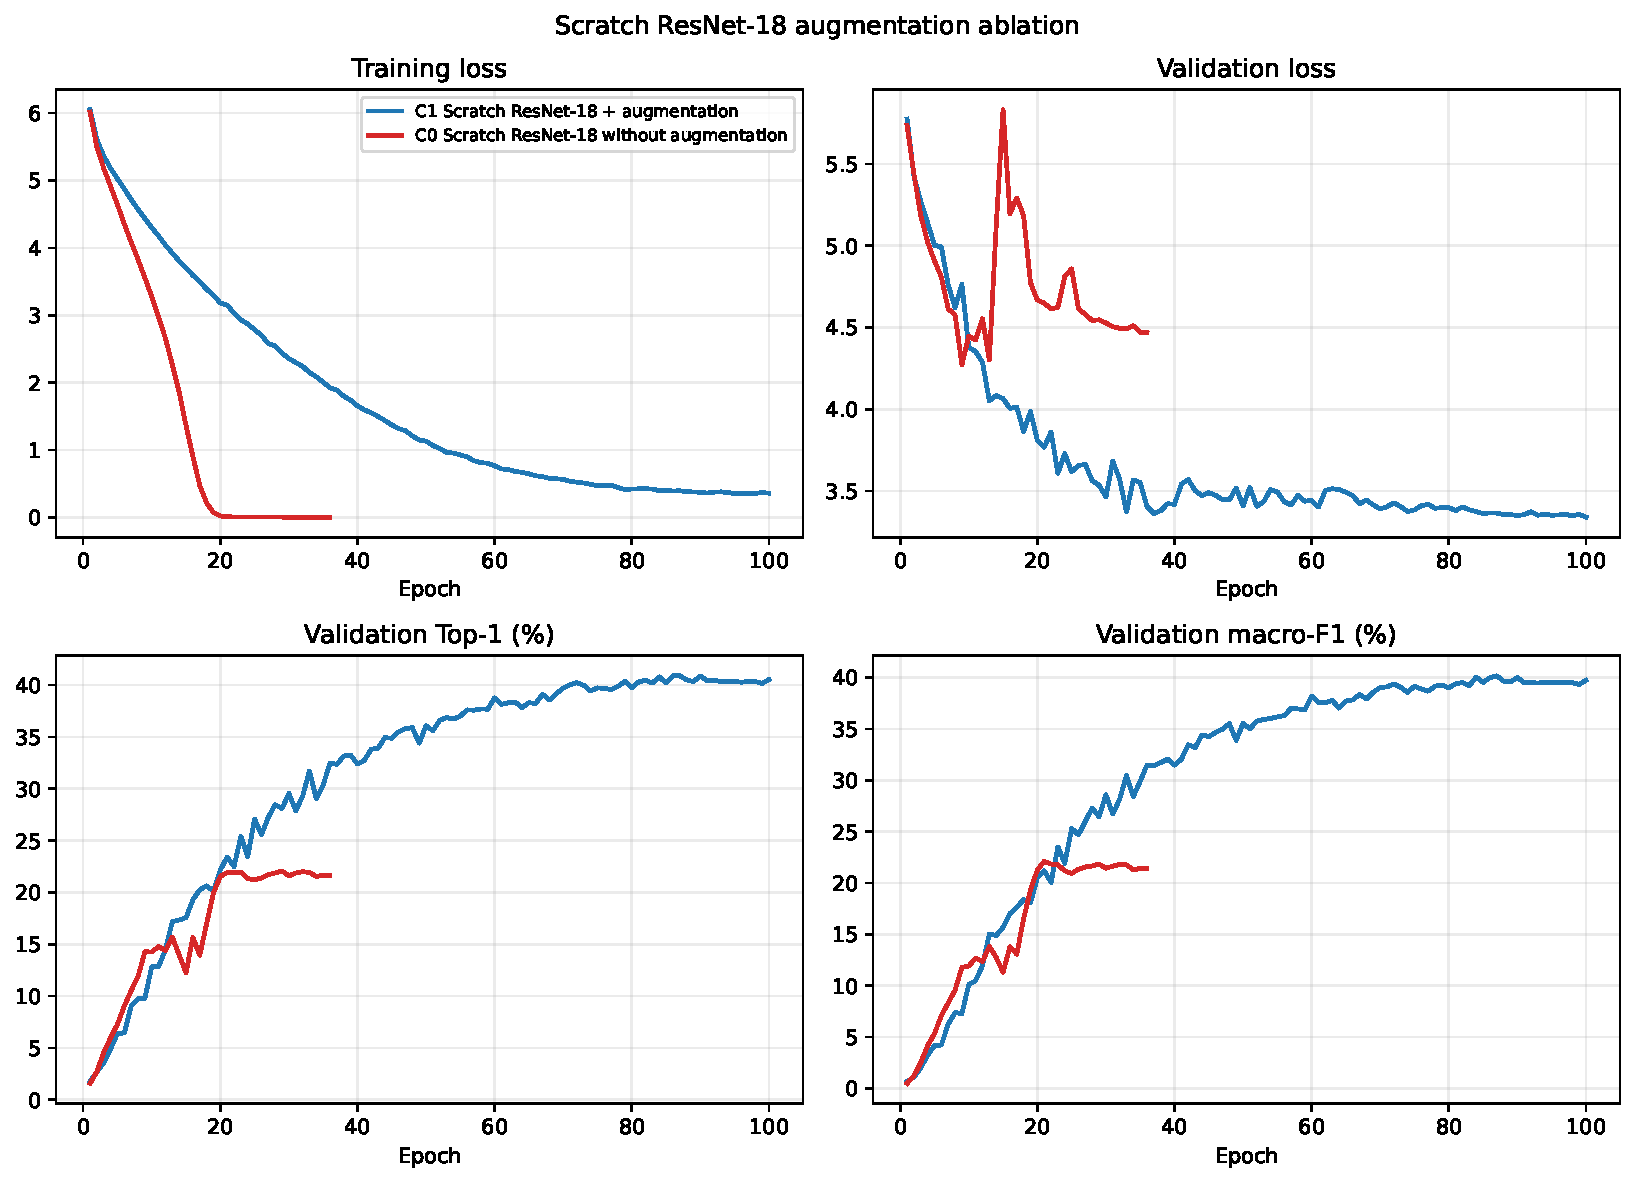
\includegraphics[width=\linewidth]{figures/c_aug_curves.pdf}
\caption{Training and validation dynamics for the controlled augmentation
ablation. C0 quickly memorises unaugmented training views and stops after
epoch 36; C1 trains for 100 epochs with much higher validation Top-1 and
macro-F1.}
\label{fig:c-curves}
\end{figure}

\subsection{Pretraining and architecture}

Pretrained ResNet-18 reaches 65.10\% test Top-1 ($\approx$45~min training;
$\approx$11.6~s inference on 5k images). EfficientNet-B0 reaches 76.66\%
Top-1 / 90.50\% Top-5 ($\approx$79~min training; $\approx$6.0~s inference).
Relative to C1 (41.32\% Top-1), ImageNet initialisation yields a large absolute
gain on the same backbone family ($+$23.8~pp Top-1 for ResNet-18); switching to
EfficientNet-B0 adds a further $+$11.6~pp under matched data and a comparable
optimisation recipe. Figure~\ref{fig:d-curves} shows training/validation
accuracy and validation macro-F1: both pretrained models improve steadily,
with EfficientNet-B0 maintaining a clear validation lead.

\begin{figure*}[t]
\centering
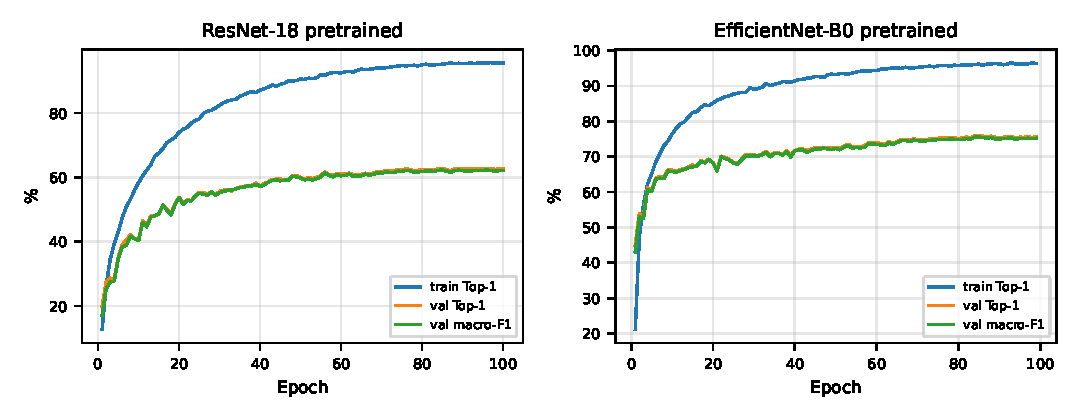
\includegraphics[width=0.95\textwidth]{figures/d_pretrain_curves.pdf}
\caption{Pretrained fine-tuning dynamics (Method~D): train/val Top-1 and
validation macro-F1 for ResNet-18 and EfficientNet-B0 over the full training
budget.}
\label{fig:d-curves}
\end{figure*}

\subsection{Timing}

Table~\ref{tab:timing} summarises representative wall-clock costs. Classical
methods spend most time extracting features or fitting linear models;
classifier-only scoring on cached BoVW vectors is sub-second for 5k images.
Deep models require GPU training on the order of tens of minutes to over an
hour per full run in our setups, with batch inference of the test set in
seconds to tens of seconds.

\begin{table}[t]
\centering
\footnotesize
\setlength{\tabcolsep}{2.5pt}
\resizebox{\columnwidth}{!}{%
\begin{tabular}{@{}lcc@{}}
\toprule
Method & Train & Test (5k) \\
\midrule
A Combined + SGD & $\approx$289~s fit & $\approx$25~s + 0.03~s \\
B BoVW SVM ($K{=}2000$) & $\approx$386~s fit & $\approx$0.04~s$^\dagger$ \\
C1 Scratch R18 + aug & 34.9~min & $\approx$6.8~s \\
D ResNet-18 pretrained & $\approx$45.1~min & $\approx$11.6~s \\
D EfficientNet-B0 & $\approx$79.1~min & $\approx$6.0~s \\
\bottomrule
\end{tabular}%
}
\caption{Approximate training and test inference times. A test time is
feature extraction + prediction. $^\dagger$B scores on cached BoVW features
(excludes SIFT/encoding).}
\label{tab:timing}
\end{table}

\subsection{Qualitative cases and Grad-CAM}

\paragraph{Handcrafted failures.}
Method~A high-scoring errors often involve small subjects with dominant sky,
foliage, or artificial texture; successes typically show a large, distinctive
organism (Figure~\ref{fig:a-cases}). Frequent validation confusions include
related plants such as \emph{Ceratiola ericoides}$\rightarrow$\emph{Calluna
vulgaris} and \emph{Sequoiadendron giganteum}$\rightarrow$\emph{Taxodium
mucronatum}, as well as occasional cross-taxon mistakes when context dominates.
Method~B high-confidence BoVW errors include cross-taxon mistakes
(e.g., damselfly$\rightarrow$cockle shell; moth$\rightarrow$bivalve),
illustrating how orderless local words can latch onto shared texture without
object identity. Correct BoVW cases include distinctive butterflies
(\emph{Papilio thoas}) and textured fungi (\emph{Xylobolus frustulatus}).
Linear SVM decision scores are used only for ranking and should not be read as
calibrated probabilities.

\paragraph{Deep confusions.}
On C1 test predictions, 2{,}066/5{,}000 images are correct and 2{,}934 are
wrong; 9 classes are perfect (10/10) and 28 classes are never recognised
(0/10). Frequent unordered confusion pairs include \emph{Aquila
heliaca}$\leftrightarrow$\emph{Pernis apivorus}, \emph{Myosotis
latifolia}$\leftrightarrow$\emph{Myosotis scorpioides}, and same-genus
\emph{Echinocereus} and \emph{Ajuga} pairs---consistent with fine-grained
biological similarity. Confusion counts alone cannot prove whether the
network uses the organism or the background; Grad-CAM addresses that below.

\paragraph{Grad-CAM.}
Figures~\ref{fig:e-correct}--\ref{fig:e-conf} show three-model Grad-CAM panels
(C1 scratch ResNet-18, pretrained ResNet-18, and EfficientNet-B0) on the same
image IDs. In correct cases, activation often covers the main organism or a
distinctive part (e.g., the bird's-nest orchid flower body), suggesting that
models can use object-relevant evidence when they are right.

\begin{figure*}[t]
\centering
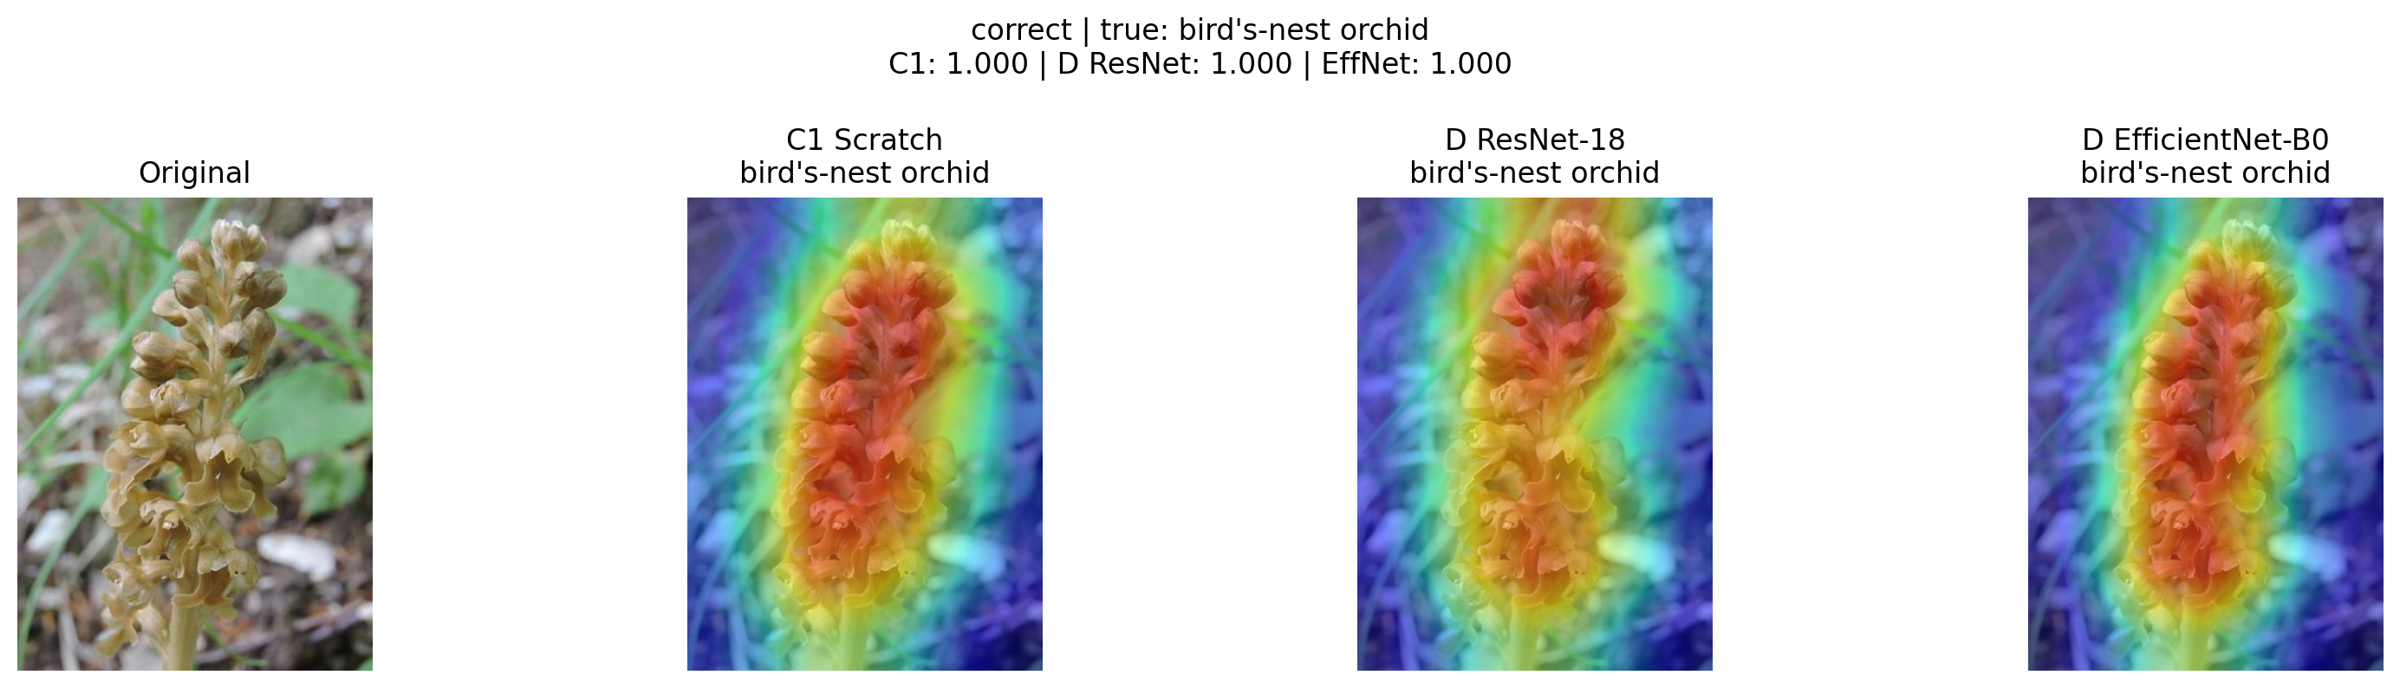
\includegraphics[width=\textwidth]{figures/e_correct_gradcam.png}
\caption{Three-model Grad-CAM for a high-confidence \emph{correct} prediction
(bird's-nest orchid / \emph{Neottia nidus-avis}). Columns show the original
image and heatmap/overlay for C1 scratch ResNet-18, pretrained ResNet-18, and
EfficientNet-B0 on the same image ID.}
\label{fig:e-correct}
\end{figure*}

In high-confidence errors, activation may still land on a salient region that
is insufficient for species identity---for example, plant-like cues when the
true class is an insect.

\begin{figure*}[t]
\centering
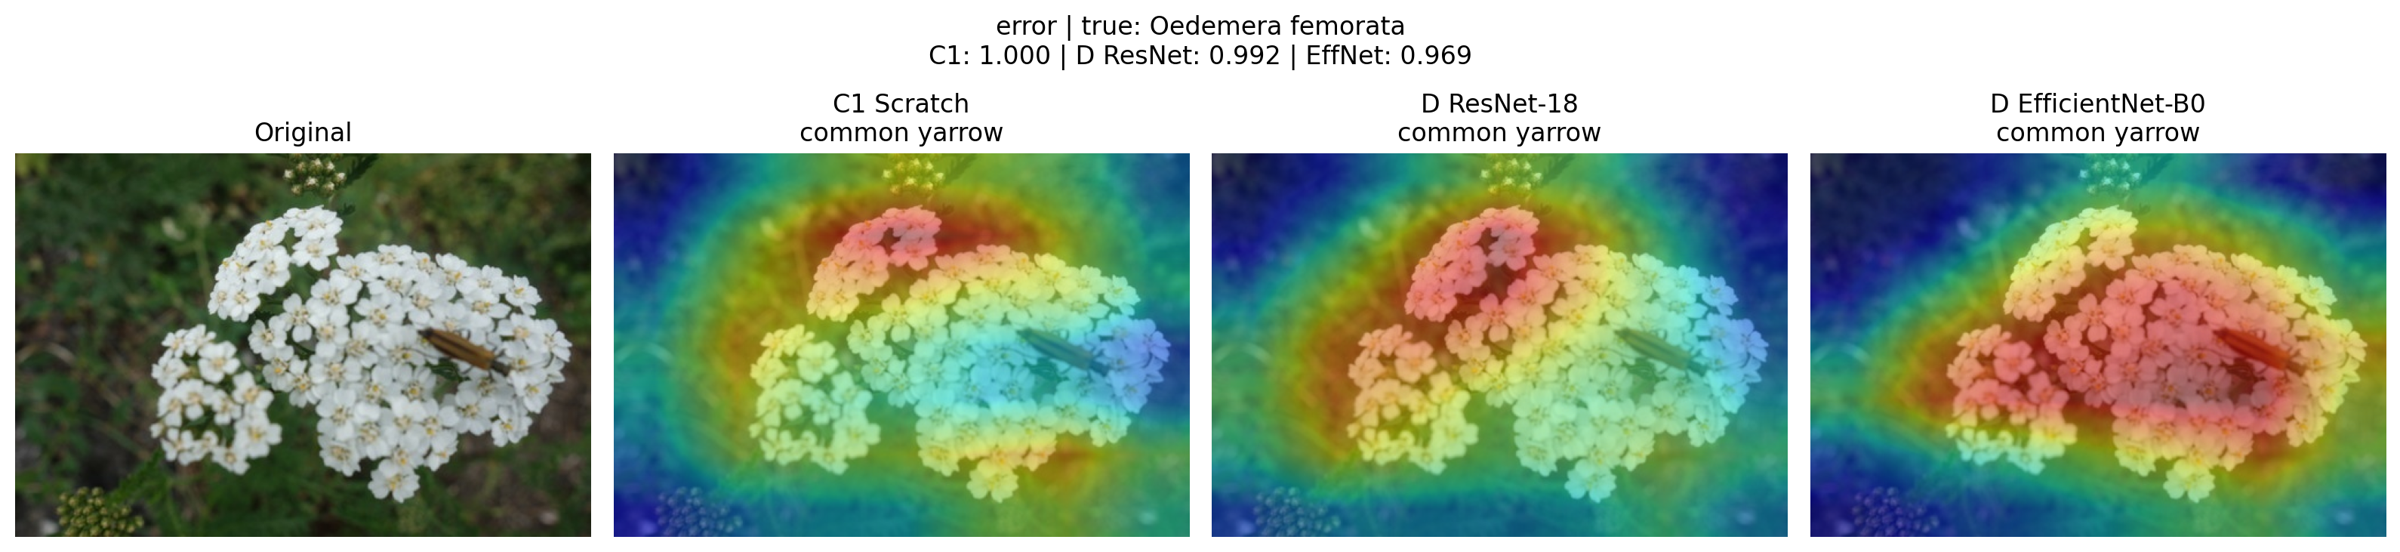
\includegraphics[width=\textwidth]{figures/e_error_gradcam.png}
\caption{Three-model Grad-CAM for a high-confidence \emph{error}: true class
\emph{Oedemera femorata}, predicted common yarrow. Salient regions need not be
species-discriminative.}
\label{fig:e-error}
\end{figure*}

For Imperial Eagle vs.\ European Honey-buzzard, heatmaps typically cover the
bird body or wings rather than empty background, yet the Accipitridae pair
remains hard because the species are visually similar. Pretrained ResNet-18 is
stronger than C1 overall; EfficientNet-B0 sometimes corrects C1 mistakes but
can still focus on strong non-discriminative cues. Layer targets differ across
architectures, so these comparisons are qualitative, not a layer-matched causal
probe.

\begin{figure*}[t]
\centering
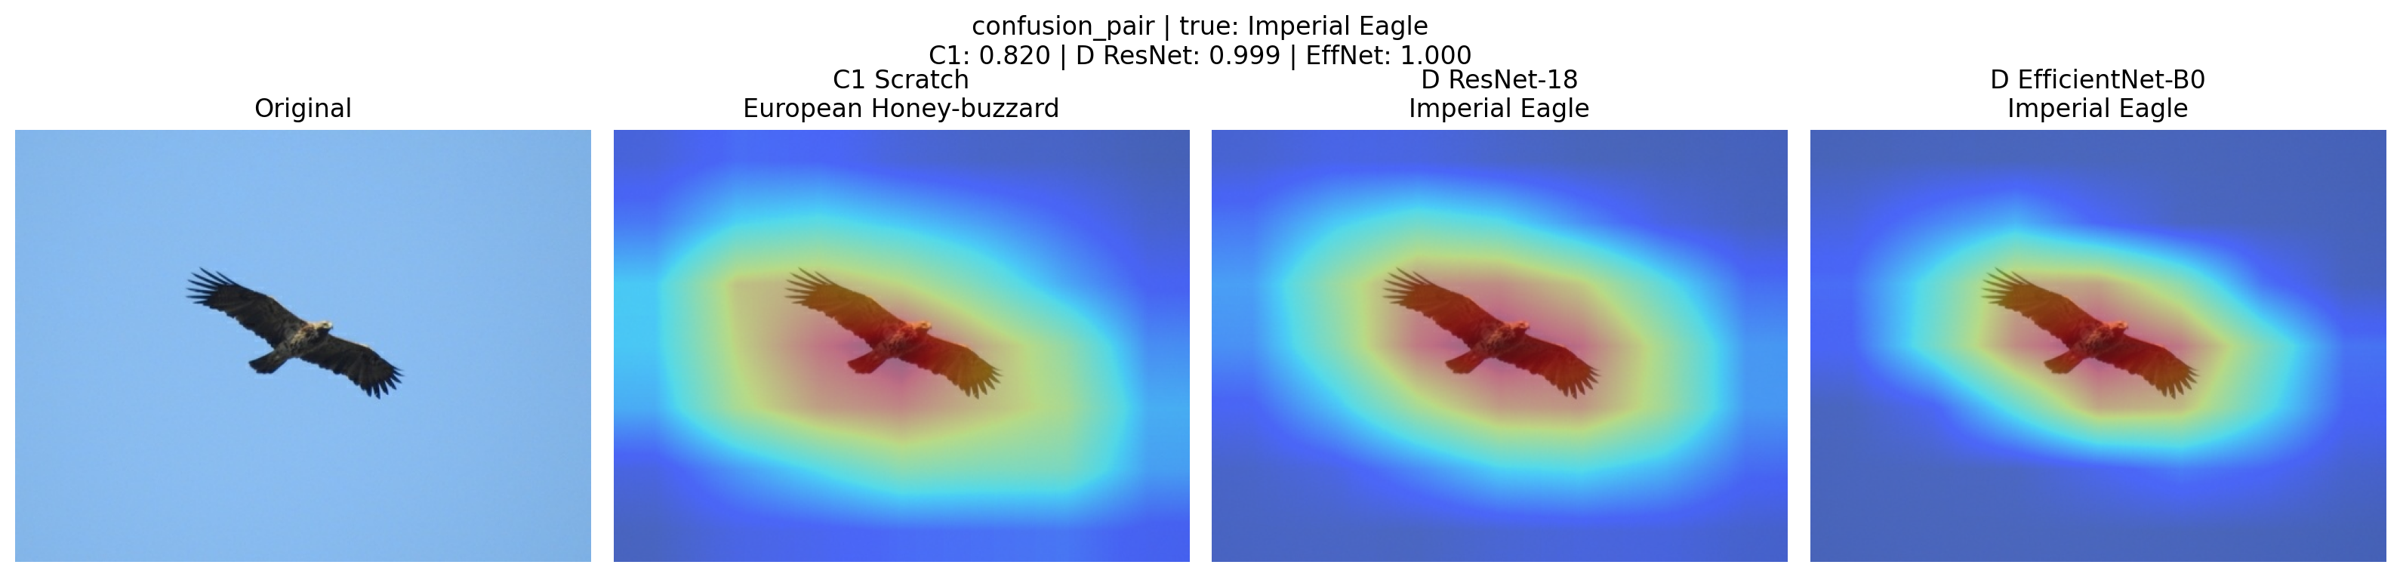
\includegraphics[width=\textwidth]{figures/e_confusion_gradcam.png}
\caption{Three-model Grad-CAM on an Imperial Eagle
(\emph{Aquila heliaca}) vs.\ European Honey-buzzard (\emph{Pernis apivorus})
confusion example. Attention is typically on the bird rather than empty
background.}
\label{fig:e-conf}
\end{figure*}

% Flush deferred figure* floats before Discussion / References.
\FloatBarrier
\clearpage

% =====================================================================
\section{Discussion}
% =====================================================================

\paragraph{Reproducibility.}
All classical and deep experiments share seed~9517, the frozen Dataset~v1.0
manifests, and the shared score evaluator. Method configurations are stored as
YAML (BoVW / scratch CNN) or JSON (pretrained runs). Grad-CAM case lists are
exported as CSV summaries so the same images can be reopened for the video
demo. Large weights and raw images are excluded from the code ZIP; notebooks
document how to attach Dataset~v1.0 and checkpoints locally.

\paragraph{Method diversity vs.\ accuracy.}
Traditional global and local descriptors exceed chance ($0.2\%$ Top-1) but
remain far behind CNNs. Descriptor ablation shows colour, LBP, and HOG are
complementary; BoVW roughly doubles Method~A Top-1 by emphasising repeatable
local patterns, yet orderless histograms still struggle with pose, part layout,
and cluttered backgrounds. Neither classical family closes the gap to learned
representations.

\paragraph{What moves the needle for CNNs.}
Basic augmentation is decisive for scratch training with only 40 images per
class: without random views, C0 almost perfectly memorises fixed training
images but generalises poorly, whereas random resized crops change organism
scale/position and flips remove a fixed orientation, forcing more invariant
features. Because C0/C1 differ only in the training transform, the large test
gap is direct single-seed evidence that these transforms help here. Pretraining
then yields a further large jump on the same backbone family, and
EfficientNet-B0 adds an architecture gain after transfer---visible both in
final metrics and in the Method~D learning curves. These controlled contrasts
cover handcrafted vs.\ deep, scratch vs.\ pretrained, and multiple CNN
architectures as required.

\paragraph{Errors are often biologically coherent.}
Method~A confusions include related plants (e.g., \emph{Ceratiola} vs.\
\emph{Calluna}) and occasional cross-taxon mistakes when background dominates.
Same-genus and same-family pairs dominate high-frequency confusions for C1,
aligning with fine-grained difficulty rather than random label noise.
Grad-CAM usually highlights organism regions on correct examples, but
high-confidence errors can attend to salient yet insufficient cues; heatmaps
are not causal evidence, and ResNet vs.\ EfficientNet layers are not matched.

\paragraph{Limitations.}
Expensive deep runs used a single seed (9517), so we avoid multi-seed
significance claims. The scratch ablation covers only random resized cropping
and horizontal flipping; richer policies may help further but would need
separate one-factor ablations. ImageNet-oriented crops and normalisation may
be suboptimal for naturalist photos. Decision scores from linear SVM
objectives are used for ranking only and are not calibrated probabilities.
Timing definitions differ across pipelines (feature extraction vs.\
classifier-only scoring vs.\ end-to-end GPU inference), so
Table~\ref{tab:timing} should be read with those caveats. We did not
exhaustively tune fine-tuning schedules (e.g., frozen backbones or
discriminative learning rates). C1 remains the scratch reference for
pretrained and Grad-CAM comparisons.

% =====================================================================
\section{Conclusion}
% =====================================================================

On a frozen 500-species iNaturalist-2021 subset, we compared handcrafted
baselines, scratch and pretrained CNNs, and Grad-CAM explanations under a
shared evaluation protocol. Global descriptors and SIFT-BoVW establish
interpretable classical baselines above chance but far below deep models.
Controlled augmentation roughly doubles scratch ResNet-18 Top-1 relative to an
unaugmented twin; ImageNet pretraining and EfficientNet-B0 yield further large
gains, reaching \textbf{76.66\%} test Top-1. Error patterns are often
taxonomically coherent, and Grad-CAM suggests organism-centred attention on
many correct cases while remaining non-causal. Future work includes multi-seed
confidence intervals, richer one-factor augmentation policies, stronger
fine-grained architectures, and tighter causal probes of model attention.

\FloatBarrier
\clearpage

{
\small
\bibliographystyle{ieeenat_abbrv}
\bibliography{main}
}

\end{document}
